% !TEX TS-program = XeLaTeX
% !TEX spellcheck = en-US
\documentclass[aspectratio=169]{beamer}

\usetheme{example}

\title{Lecture 1: \\ Introduction and working with data}
\institute{GRA 4160: Predictive Modelling with Machine Learning}
\date{January 16th 2025}
\author{Vegard H\o ghaug Larsen}

\begin{document}

\maketitle

\frame{
	\frametitle{About me:}
	Vegard H\o ghaug Larsen (Department of Data Science and Analytics)\\
	Background: PhD in Economics followed by six years in Norges Bank
	$\;$\\
	Email: vegard.h.larsen@bi.no\\
	%$\;$\\
	%Office hours: Wednesday 13:00-15:00 (or by appointment)\\
	$\;$\\
	Office: B3Y-075
}

\frame{
    \frametitle{Syllabus}


    \begin{minipage}{0.65\textwidth}
        The textbook for this course is:\\
        \begin{enumerate}
            \item[] \textit{The Elements of Statistical Learning: Data Mining, Inference, and Prediction} by \textit{Trevor J. Hastie; Robert J. Tibshirani; Jerome Friedman}
            (\href{https://hastie.su.domains/Papers/ESLII.pdf}{Link})
        \end{enumerate}
    \end{minipage}
	\hfill
	\begin{minipage}{0.3\textwidth}
        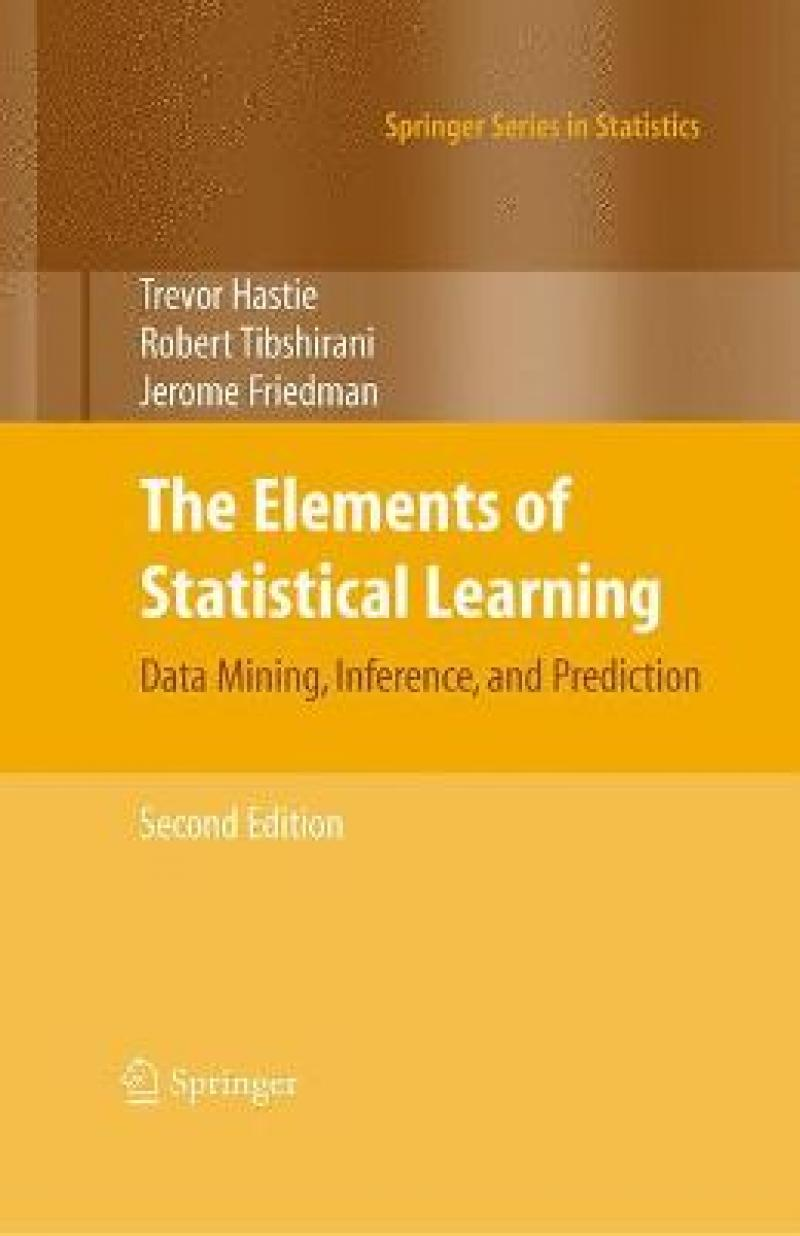
\includegraphics[width=0.5\textwidth]{figures/ESL.jpg} % Replace with the path to the image of the first book
    \end{minipage}

    \bigskip

    \begin{minipage}{0.3\textwidth}
        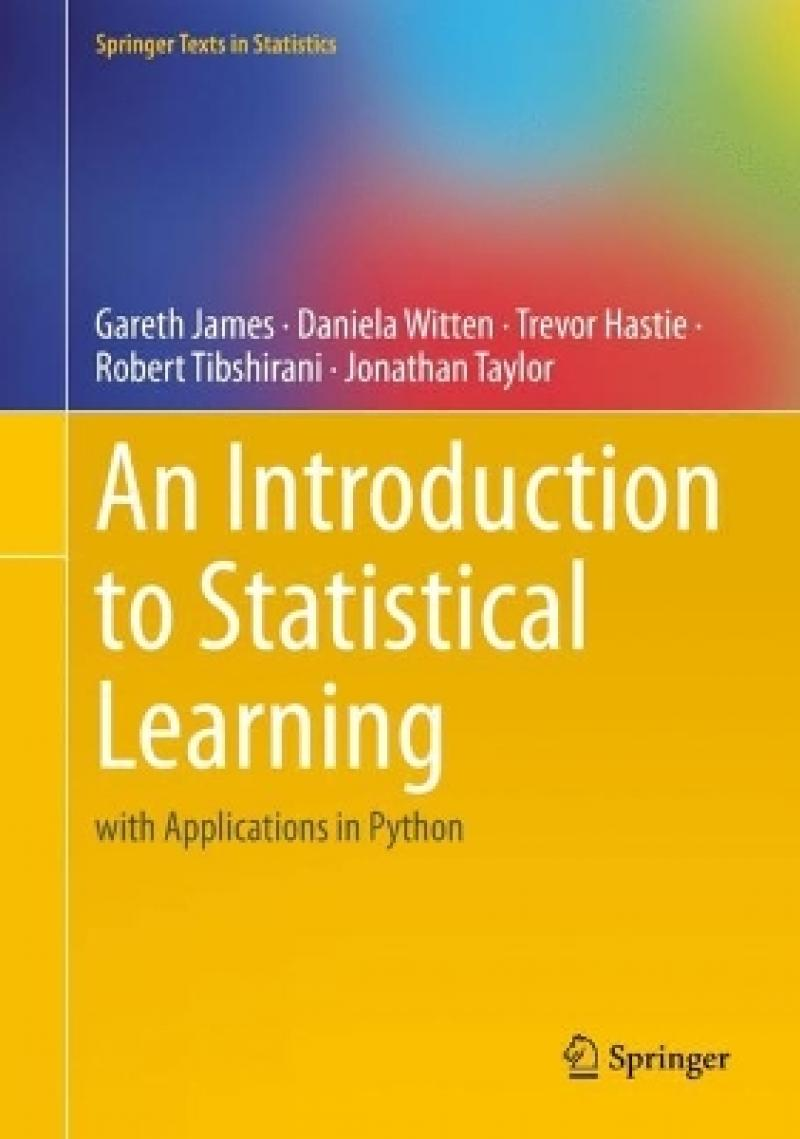
\includegraphics[width=0.5\textwidth]{figures/ISL.jpg} % Replace with the path to the image of the second book
    \end{minipage}
    \hfill
    \begin{minipage}{0.65\textwidth}
        For a more gentle introduction to many of the same subjects, I recommend the following book:\\
        \begin{enumerate}
            \item[] \textit{An Introduction to Statistical Learning} by \textit{Gareth James; Daniela Witten; Trevor Hastie; Robert Tibshirani}
            (\href{https://www.statlearning.com/}{Link})
        \end{enumerate}
    \end{minipage}
}

\frame{
	\frametitle{Prerequisites / What I Expect You to Know}

	\begin{itemize}
		\item \textbf{Mathematics:} Basic linear algebra and multivariate calculus
		\item \textbf{Statistics:} Fundamental probability and statistical concepts
		\item \textbf{Python Programming:} Experience with NumPy, Pandas, and Matplotlib
		\item \textbf{Object-Oriented Programming:} Ability to write and understand OOP structures in Python
	\end{itemize}
}


\frame{
	\frametitle{About this Course}

	\begin{itemize}
		\item Focused on \textbf{predictive modeling} using traditional (pre-deep learning) machine learning methods.
		\item Covers fundamental algorithms such as linear and logistic regression, decision trees, and ensemble methods.
		\item Emphasis on \textbf{hands-on practice}: you will write code from scratch to implement and understand key algorithms.
		\item Provides practical insights into common workflows: data preprocessing, model training, hyperparameter tuning, and model evaluation.
		\item Prepares you to critically evaluate and improve models for real-world predictive tasks.
	\end{itemize}
}


\frame{
\frametitle{Mini Project}

\begin{itemize}
	\item \textbf{Group Work:} Form groups of 2--4 students. I will add a excel sheet on itslearning that you should use to form groups within next week. 
	\item \textbf{Objective:} Apply the learned methods to a real-world data problem on a smaller scale.
	\item \textbf{Feedback Sessions:} Each group can schedule up to two meetings (in-person or via Zoom) for guidance and feedback.
	\item \textbf{Presentation:} Present your work to the class at the end of the semester.
	\item \textbf{Documentation:} (Optional but recommended) Use a GitHub repository to share code and a short project report.
	\item \textbf{Evaluation:} The project is graded (letter grade) and accounts for 30\% of the final grade.
	\item \textbf{Exam Integration:} Be prepared to answer related questions during the final exam.
\end{itemize}
}


\frame{
\frametitle{Course Structure}

\begin{itemize}
	\item \textbf{Interactive Format:} Lectures will be as interactive as possible, minimizing traditional lecture-style teaching.
	\item \textbf{Topic Introductions:} I will often start with a few slides to introduce a concept, then focus on live coding, examples, and exercises.
	\item \textbf{Course Materials:} Expect one to two notebooks with background materials and one exercise notebook per session.
	\item \textbf{Pre-class Preparation:} All notebooks will be available on Itslearning before each class, and you are expected to review them in advance.
	\item \textbf{Project Guidance:} We will also devote time in some lectures to discuss the mini project and offer guidance on your approach.
\end{itemize}
}


\frame{
	\frametitle{Using Generative AI as a Learning Tool}

	\begin{itemize}
		\item Generative AI is a powerful resource for exploration, idea generation, and problem-solving.
		\item Treat it as a learning partner rather than a replacement for your own reasoning skills.
		\item Use it to enhance your understanding, spark creativity, and experiment with new approaches.
		\item Focus on leveraging it as a supportive tool: ask questions, seek clarifications, and discover alternative solutions.
		\item You can access \textbf{GPT-UiO}, a GDPR-compliant platform provided by UiO, for free.
		\item \textbf{GitHub Copilot} is also recommended. You should be able to get an educational license for free.
		\item Always apply critical thinking, ethical considerations, and proper attribution when using these tools.
	\end{itemize}
}

\frame{
    \frametitle{Use an Integrated Development Environment (IDE)}
    \textbf{Why use an IDE?}
    \begin{itemize}
        \item Simplifies coding by integrating essential tools in one interface.
        \item Enhances productivity with features like syntax highlighting, debugging, and extensions.
    \end{itemize}

    \vspace{1em}
    \textbf{Why Visual Studio Code (VSCode)?}
    \begin{itemize}
        \item \textbf{Lightweight yet powerful:} Supports many programming languages and frameworks.
        \item \textbf{Extensions:} Customize your environment with thousands of extensions (e.g., Python, Jupyter).
        \item \textbf{Version Control:} Integrated Git support makes it easy to collaborate and track changes.
        \item \textbf{Built-in terminal:} Run commands and scripts directly within the editor.
        \item \textbf{Cross-platform:} Works seamlessly on Windows, macOS, and Linux.
    \end{itemize}

    \vspace{1em}
    \textbf{Ideal for students:} VSCode is free, beginner-friendly, and widely used in the industry. As a student you might also be eligible for a free GitHub Copilot account.
}


\frame{
	\frametitle{About You}
	\begin{itemize}
		\item Please introduce yourself: What is your name and your academic/professional background?
		\pause
		\item Do you have any specific career goals related to data science, analytics, or machine learning?
		\pause
		\item What are your main learning objectives or expectations for this course?
		\pause
		\item Are there any questions or concerns you have about the course structure, topics, or logistics?
	\end{itemize}
}


\frame{
	\frametitle{Plan for Today}
	
	\underline{\bf Working with Data in Jupyter Notebooks:}
	
	\begin{itemize}
		\item Understand why \textbf{Jupyter notebooks} have become a standard tool for data exploration and ML prototyping.
		\item Recognize that \textbf{data preprocessing} (cleaning, transforming, encoding, and scaling) is essential for high-quality predictive modeling.
		\item Learn how to systematically apply preprocessing techniques in Python, ensuring reproducibility and consistency across projects.
		\item Gain hands-on experience implementing common techniques (handling missing values, encoding categories, scaling features) to prepare data for modeling.
	\end{itemize}
	
	\bigskip
	\pause

	\underline{\bf Material:}
	\begin{itemize}
		\item Lecture Notebook: \texttt{01\_Working\_with\_data\_in\_jupyter\_notebooks.ipynb}
		\item Exercise Notebook: \texttt{01\_Data\_preprocessing\_titanic.ipynb}
	\end{itemize}
}

\frame{
    \frametitle{Machine Learning Workflow}
    \begin{itemize}
        \item \textbf{Define the problem and collect data:} Clarify your predictive task and gather relevant data.
        \item \textbf{Data preprocessing:} Clean, transform, and encode data to ensure quality and consistency.
        \item \textbf{Model selection:} Choose appropriate algorithms (e.g., linear regression, decision trees, ensembles).
        \item \textbf{Training and tuning:} Fit models and tune hyperparameters using appropriate metrics.
        \item \textbf{Evaluation and deployment:} Evaluate performance on unseen data and integrate the model into real-world applications.
    \end{itemize}
}

\frame{
    \frametitle{Traditional ML vs. Deep Learning}
    \begin{itemize}
        \item \textbf{Feature Engineering:}
        \begin{itemize}
            \item \textit{Traditional ML:} Often requires manual feature engineering (domain knowledge, handcrafted features).
            \item \textit{Deep Learning:} Learns representations directly from raw data (images, text, etc.).
        \end{itemize}
        \item \textbf{Data Requirements:}
        \begin{itemize}
            \item \textit{Traditional ML:} Performs well with smaller datasets; structured data often sufficient.
            \item \textit{Deep Learning:} Typically needs large datasets and significant computational resources.
        \end{itemize}
        \item \textbf{Model Complexity:}
        \begin{itemize}
            \item \textit{Traditional ML:} Simpler models like SVM, decision trees, linear models.
            \item \textit{Deep Learning:} Neural networks with multiple layers (CNNs, RNNs, Transformers).
        \end{itemize}
        \item \textbf{Interpretability:}
        \begin{itemize}
            \item \textit{Traditional ML:} Models like linear/logistic regression can be straightforward to interpret.
            \item \textit{Deep Learning:} Deep networks can be more opaque, requiring specialized interpretation methods.
        \end{itemize}
    \end{itemize}
}

\frame{
    \frametitle{Overfitting vs. Underfitting}
    \begin{itemize}
        \item \textbf{Overfitting:}
        \begin{itemize}
            \item Model fits noise in the training data, failing to generalize.
            \item Symptoms: Very low training error, high validation/test error.
            \item Remedies: More data, regularization, dropout (in NN), simpler model.
        \end{itemize}
        \item \textbf{Underfitting:}
        \begin{itemize}
            \item Model is too simple to capture the underlying trend.
            \item Symptoms: High training error, high validation/test error.
            \item Remedies: More complex model, adding features, reducing regularization.
        \end{itemize}
    \end{itemize}
}

\frame{
    \frametitle{Train, Validation, and Test Splits}
    \begin{itemize}
        \item \textbf{Training Set:}
        \begin{itemize}
            \item Used to fit the parameters of your model.
        \end{itemize}
        \item \textbf{Validation Set:}
        \begin{itemize}
            \item Used for hyperparameter tuning and model selection.
            \item Prevents overfitting to the training set.
        \end{itemize}
        \item \textbf{Test Set:}
        \begin{itemize}
            \item Used only for the final evaluation.
            \item Mimics "unseen data" in the real world.
        \end{itemize}
        \item \textbf{Key Point:}
        \begin{itemize}
            \item Proper splitting strategies (e.g., random splits, stratification, cross-validation) are crucial for reliable performance estimates.
        \end{itemize}
    \end{itemize}
}

\frame{
    \frametitle{Interpreting Model Results}
    \begin{itemize}
        \item \textbf{Performance Metrics:} Use appropriate metrics (MAE, RMSE, F1-score, AUC) depending on the problem type.
        \item \textbf{Visual Diagnostics:} Confusion matrices, ROC curves, residual plots provide deeper insights.
        \item \textbf{Explainability Tools:} Techniques like SHAP help interpret complex models.
        \item \textbf{Domain Knowledge:} Model results are more meaningful if interpreted in the context of the application area.
        \item \textbf{Communication:} Clearly communicate strengths, weaknesses, and uncertainties to stakeholders.
    \end{itemize}
}

\frame{
    \frametitle{Why Genuine Learning Matters in an AI-Powered World}
    \textbf{Unlimited Resources, Home Exam:} You can use all available tools, including Generative AI models. \\
    \bigskip

    \textbf{But why understand the material?}
    \begin{itemize}
        \item \textbf{Long-Term Skill Building:} Real expertise isn't just about getting the right answer today—it’s about being able to solve unseen problems tomorrow.
        \item \textbf{Critical Thinking:} Understanding how a solution is derived helps you detect AI mistakes and evaluate outcomes thoughtfully.
        \item \textbf{Career Readiness:} Employers value people who can interpret and adapt AI-generated results, not just copy and paste them.
        \item \textbf{Exam Rigor:} We will ask you to \emph{explain and justify} steps, ensuring you can interpret AI-produced solutions. 
    \end{itemize}
}

\frame{
    \frametitle{My expectations:}
    
    \begin{itemize}
        \item Engage actively with the course materials, exercises, and discussions.
        \item Be ready to \textit{talk through your solutions} and justify each step logically.
        \item Ultimately, \textbf{your genuine knowledge} is what matters most.
    \end{itemize}
}

\end{document}